\documentclass[tikz,border=8pt]{standalone}
\usepackage{amsmath}
\usetikzlibrary{arrows.meta,calc}
\definecolor{ink}{HTML}{21352F}\definecolor{teal}{HTML}{087F7B}
\definecolor{blue}{HTML}{4B77A8}\definecolor{gold}{HTML}{C58B2A}
\begin{document}
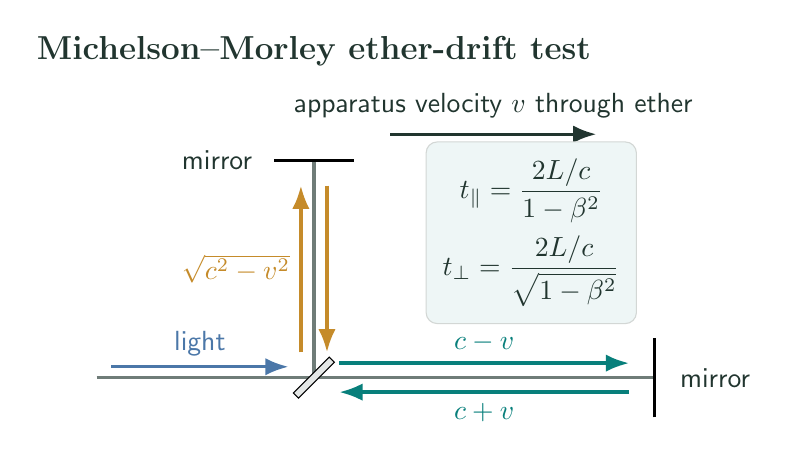
\begin{tikzpicture}[font=\sffamily,text=ink,>=Latex,scale=.92]
  \node[font=\bfseries\large] at (0,4.5) {Michelson--Morley ether-drift test};
  \coordinate (B) at (0,0); \coordinate (P) at (4.7,0); \coordinate (T) at (0,3);
  \draw[very thick,ink!65] (-3,0)--(P);
  \draw[very thick,ink!65] (B)--(T);
  \draw[fill=ink!12,rotate around={45:(B)}] (-.35,-.05) rectangle (.35,.05);
  \draw[very thick] ($(P)+(0,-.55)$)--($(P)+(0,.55)$);
  \node[anchor=west] at ($(P)+(.22,0)$) {mirror};
  \draw[very thick] ($(T)+(-.55,0)$)--($(T)+(.55,0)$);
  \node[anchor=east] at ($(T)+(-.72,0)$) {mirror};
  \draw[blue,very thick,->] (-2.8,.15)--(-.35,.15) node[midway,above] {light};
  \draw[teal,very thick,->] (.35,.2)--(4.35,.2) node[midway,above] {$c-v$};
  \draw[teal,very thick,->] (4.35,-.2)--(.35,-.2) node[midway,below] {$c+v$};
  \draw[gold,very thick,->] (-.18,.35)--(-.18,2.65) node[midway,left] {$\sqrt{c^2-v^2}$};
  \draw[gold,very thick,->] (.18,2.65)--(.18,.35);
  \draw[->,very thick,ink] (1.05,3.36)--(3.9,3.36)
    node[midway,above=2pt] {apparatus velocity $v$ through ether};
  \node[draw=ink!20,fill=teal!7,rounded corners=4pt,align=center,inner sep=6pt] at (3.0,2.0)
    {$t_\parallel=\dfrac{2L/c}{1-\beta^2}$\\[4pt]$t_\perp=\dfrac{2L/c}{\sqrt{1-\beta^2}}$};
\end{tikzpicture}
\end{document}
